\documentclass[11pt]{article} 



\makeatletter
\renewcommand\section{\@startsection{section}{1}{\z@}%
                                  {-3.5ex \@plus -1ex \@minus -.2ex}%
                                  {2.3ex \@plus.2ex}%
                                  {\normalfont\large\bfseries}}
\makeatother

\addtolength{\oddsidemargin}{-.875in}
\addtolength{\evensidemargin}{-.875in}
\addtolength{\textwidth}{1.75in}
\addtolength{\topmargin}{-.875in}
\addtolength{\textheight}{1.75in}


\usepackage{amssymb}
\usepackage{amsmath}
\usepackage{amsthm}
\usepackage{graphicx,caption,subcaption}


\usepackage{titling}
\setlength{\droptitle}{-6em}
\posttitle{\par\end{center}\vspace{-4.8em}}

\newcommand{\R}{{\ensuremath{\mathbb{R}}} }
\newcommand{\Q}{{\ensuremath{\mathbb{Q}}} }
\newcommand{\C}{{\ensuremath{\mathbb{C}}} }
\newcommand{\N}{{\ensuremath{\mathbb{N}}} }
\newcommand{\Z}{{\ensuremath{\mathbb{Z}}} }

\newcommand{\sexion}{\addtocounter{section}{1} }


\newcommand{\hint}[1]{{(\emph{Hint:} #1)}} %This line shows hints
%\newcommand{\hint}[1]{} %Use this line to hide all hints


\usepackage{fancyhdr}
\pagestyle{fancyplain}
\renewcommand{\headrulewidth}{0pt}

\begin{document}

%\lhead{}
\rhead{Mixing Example}

Recall that at the end of our last problem we had a 50 gallon container completely full of salt water. There were 21 lbs of salt in the container, and water was continuing to pour in at a rate of 4 gal/min, .5 lbs salt / gal. 

\[\frac{dx}{dt} = (\mathrm{rate\ in}) - (\mathrm{rate\ out})\]
\[\frac{dx}{dt} = \left( 4 \frac{\mathrm{gal}}{\mathrm{min}}\right) \cdot \left( \frac{1}{2} \frac{\mathrm{lbs}}{\mathrm{gal}} \right)- \left( 4 \frac{\mathrm{gal}}{\mathrm{min}}\right)  \frac{x}{50}\]
\[\frac{dx}{dt} = 2 - \frac{2}{25} x\]

We can solve by separation of variables
\[\frac{dx}{dt} = 2 - \frac{2}{25} x\]
\[\frac{1}{2 - \frac{2}{25} x } dx = dt\]
\[- \frac{25}{2} \left( \frac{1}{  x - 25 } \right) dx = dt\]
\[- \frac{25}{2}  \int \frac{1}{  x - 25 }  dx = \int dt\]
\[- \frac{25}{2} \log (  x - 25 )   = t + C\]
\[  (  x - 25 )^{- \frac{25}{2}}   =  Ce^t\]
\[   x - 25   =  Ce^{- \frac{2}{25} t } \]
\[   x = 25 +  Ce^{- \frac{2}{25} t } \]

Since we started out with 21 lbs of salt in the tank, $x(0) = 18$ and we can find $C$.
\[   x(0)=21  = 25 +  Ce^{- \frac{2}{25} \cdot 0 } \Rightarrow 21 = 25 + C \Rightarrow C = -4\]
and the final solution is
\[x(t) = 25 - 4 e ^{- \frac{2}{25} t } \]
\[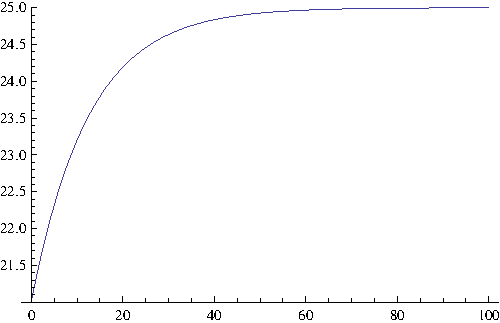
\includegraphics{MixingFigure1}\]
\center{A plot of salt content as a function of time for the first 100 minutes.}






Recall that in the previous problem, the salt content was given by 
\[x_1(t) = \frac{t(t+20)}{t+10}\]
until $t=15$ when it became full. We can shift our new solution over by 15 minutes as
\[x_2(t) = x(t-15) = 25 - 4e ^{-\frac{2}{25} (t-15)}\]
Now we have a complete description of the amount of salt
\[\left\{ \begin{array}{ll} x_1 & 0 \leq x \leq 15 \\ x_2 & x> 15 \end{array}\right.\]
\[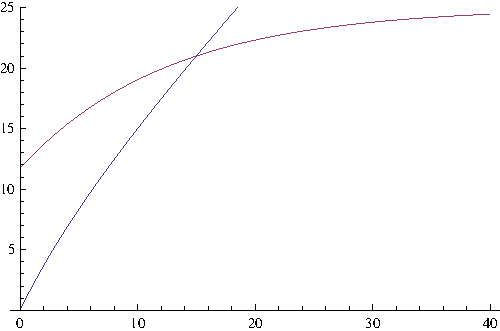
\includegraphics{MixingFigure2}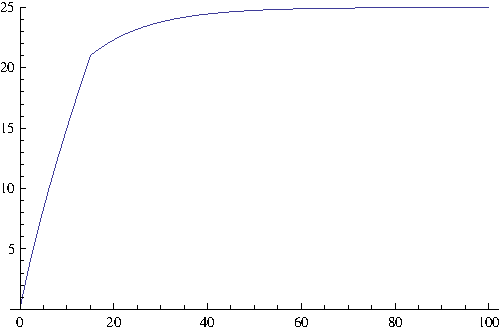
\includegraphics{MixingFigure3}\]
\center{Plots of $x_1,x_2$, and the amount of salt respectively}








\end{document}
